\section{Results}
\label{sec:results}

\paragraph{Validity checks.}
All 16{,}234 Jev calls and all local predictions returned a valid probability vector: no request failed after retries
and no input was refused, including on HateXplain. On the 970-example FPB test set that \citet{deusser2026jev} also use,
Jev's accuracy is 0.744, consistent with the 0.730 they report. Full-data DeBERTa-v3-large reaches 0.976 accuracy on
TREC-6, close to the 0.974 reported for fully fine-tuned RoBERTa-large \citep{gao2021making}, and 0.703 Macro-F1 on
HateXplain, slightly above the best value we found reported for that test split, 0.699 \citep{kim2022why}. The four local
models gave identical probabilities when 50 CLINC150 development examples were scored twice. Jev is not: in four runs over the same 500 test examples per dataset, it returned the same
prediction for 96.4--99.8\% of examples but the same probability vector for only 19.4--87.4\% of them, with differences of
up to 0.29 between runs; its ECE on these subsets varied by at most 0.012 between runs (\hyperref[app:results]{Appendix~\ref*{app:results}}). All
analyses use a single full run of each system.

\paragraph{Overview.}
\hyperref[tab:exp1]{Table~\ref*{tab:exp1}} gives the test-set results without shift. Full-data DeBERTa-v3-large has the highest Macro-F1 point
estimate on all five datasets, although Jev is within 0.3~points on CLINC150. Among the zero-shot systems in
\hyperref[tab:exp1]{Table~\ref*{tab:exp1}}, Jev has the highest Macro-F1 point estimate on every dataset (by 0.3~points over Qwen3.5-9B on
FPB). No zero-shot system is reliable on HateXplain (Macro-F1 at most 0.514), where even TF-IDF reaches 0.645.
Calibration varies more by task than by system class: ECE is at most 0.020 for all zero-shot systems on CLINC150, but
between 0.214 and 0.340 on HateXplain. These comparisons are descriptive; the tested comparisons follow.

\begin{table}[t]
  \centering
  \caption{\textbf{Full-data DeBERTa-v3-large has the highest Macro-F1 point estimate on every dataset, and the
  calibration of zero-shot systems depends more on the task than on the system.} Test-set Macro-F1 and ECE (15 bins,
  top label), candidate-restricted, no shift. These are point estimates; tested comparisons are in
  \hyperref[fig:pairs]{Figure~\ref*{fig:pairs}} and \hyperref[tab:pa]{Table~\ref*{tab:pa}}.}
  \label{tab:exp1}
  \scriptsize
  \setlength{\tabcolsep}{3pt}
  \begin{tabular}{lrrrrrrrrrr}
\toprule
 & \multicolumn{2}{c}{CLINC150} & \multicolumn{2}{c}{HWU64} & \multicolumn{2}{c}{FPB} & \multicolumn{2}{c}{HateXplain} & \multicolumn{2}{c}{TREC-6} \\
\cmidrule(lr){2-3} \cmidrule(lr){4-5} \cmidrule(lr){6-7} \cmidrule(lr){8-9} \cmidrule(lr){10-11}
System & F1$\uparrow$ & ECE$\downarrow$ & F1$\uparrow$ & ECE$\downarrow$ & F1$\uparrow$ & ECE$\downarrow$ & F1$\uparrow$ & ECE$\downarrow$ & F1$\uparrow$ & ECE$\downarrow$ \\
\midrule
\multicolumn{11}{l}{\textsc{Typed decision models}} \\
Jev & 0.978 & 0.007 & 0.908 & 0.036 & 0.752 & 0.095 & 0.514 & 0.279 & 0.922 & 0.042 \\
Tev1-4B & 0.964 & 0.008 & 0.895 & 0.040 & 0.735 & 0.072 & 0.458 & 0.214 & 0.889 & 0.038 \\
Nimble-9B & 0.962 & 0.008 & 0.896 & 0.035 & 0.629 & 0.263 & 0.470 & 0.336 & 0.872 & 0.043 \\
\midrule
\multicolumn{11}{l}{\textsc{Base LLMs}} \\
Qwen3.5-4B & 0.939 & 0.011 & 0.866 & 0.058 & 0.635 & 0.204 & 0.441 & 0.247 & 0.882 & 0.037 \\
Qwen3.5-9B & 0.955 & 0.020 & 0.884 & 0.078 & 0.749 & 0.168 & 0.487 & 0.340 & 0.903 & 0.061 \\
\midrule
\multicolumn{11}{l}{\textsc{Trained classifiers (full data)}} \\
DeBERTa-v3-large & 0.980 & 0.013 & 0.939 & 0.030 & 0.870 & 0.111 & 0.703 & 0.141 & 0.971 & 0.021 \\
TF-IDF + LR & 0.950 & 0.015 & 0.900 & 0.098 & 0.693 & 0.167 & 0.645 & 0.069 & 0.891 & 0.071 \\
\bottomrule
\end{tabular}

\end{table}

\subsection{RQ1: What decision training changes}
\label{sec:rq1}

\paragraph{Decision training improves the 9B backbone's calibration on intent tasks and lowers its Macro-F1 on financial
sentiment by 12~points.}
Nimble-9B differs from Qwen3.5-9B only by a LoRA adapter: the base weights, 8-bit precision, prompts and readout are
identical. On CLINC150 the adapter lowers ECE by 1.2~points (95\% CI $[-1.5,-0.6]$; Holm-adjusted $p<0.007$) and raises
Macro-F1 by 0.7~points ($[0.2, 1.2]$; $p=0.029$). On HWU64 it lowers ECE by 4.2~points ($[-5.6,-2.5]$; $p<0.007$). On FPB,
by contrast, Nimble-9B's Macro-F1 is 12.0~points below its base ($[-14.6,-9.3]$; $p<0.007$) and its ECE is 9.6~points
higher ($[6.8, 12.1]$; $p<0.007$). On HateXplain and TREC-6 neither difference is significant after correction; the
largest of these, $-3.1$ Macro-F1~points on TREC-6, has an interval of $[-7.0, 0.7]$ (\hyperref[fig:pairs]{Figure~\ref*{fig:pairs}}).

\paragraph{Tev1-4B is never significantly worse than its base model.}
Tev1-4B's Macro-F1 is higher than Qwen3.5-4B's on CLINC150 ($+2.5$, $[1.9, 3.1]$; $p<0.007$), HWU64 ($+2.8$,
$[1.1, 4.8]$; $p=0.040$) and FPB ($+10.0$, $[7.4, 12.7]$; $p<0.007$), and its ECE is lower on FPB ($-13.2$,
$[-15.7,-10.4]$; $p<0.007$) and HateXplain ($-3.2$, $[-5.2,-1.4]$; $p=0.029$). None of the ten differences favours the
base model significantly. Because Tev1 is a full fine-tune whose exact base revision and recipe are not published, and
because the 18--22 options of the intent datasets lie outside its training distribution, this pair is the closest
available comparison rather than a controlled one. On HWU64, 614 of the 1{,}076 test texts also occur in MASSIVE
\citep{fitzgerald2023massive}; on the 462 remaining examples every system, including the trained classifiers, loses 2.2
to 5.9 Macro-F1~points, the P2 calibration result holds ($-4.3$ ECE points, $[-5.8,-1.1]$), and the P1 Macro-F1
difference keeps its sign but is no longer resolved ($+3.0$, $[-0.03, 8.3]$; exploratory, \hyperref[tab:hwu64]{Table~\ref*{tab:hwu64}}).

The two pairs thus point in opposite directions on FPB: Tev1-4B scores 10.0 Macro-F1~points above its base, and
Nimble-9B 12.0~points below its own. Nimble-9B's loss is concentrated on the neutral class: it labels 285 of the 565
neutral test sentences as positive, against 159 for Qwen3.5-9B, so that its recall on neutral sentences falls from 0.64
to 0.36 while its recall on positive and negative sentences rises (0.88 to 0.96 and 0.89 to 0.95; descriptive,
\hyperref[tab:fpbconf]{Table~\ref*{tab:fpbconf}}). A later Nimble release, whose training data include public TREC questions, scores
0.963 Macro-F1 on TREC-6 against 0.872 for the release we test (exploratory; \hyperref[app:results]{Appendix~\ref*{app:results}}), which
suggests that the training data, not only decision training, affect the result.

\begin{figure}[t]
  \centering
  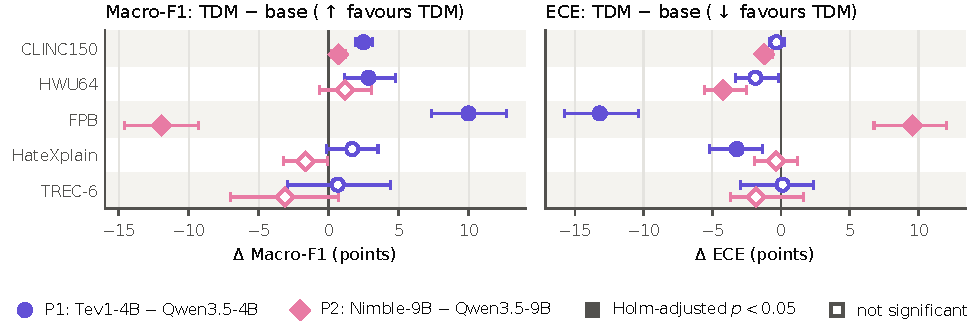
\includegraphics[width=\linewidth]{figures/fig2_pairs.pdf}
  \caption{\textbf{Tev1-4B is never significantly worse than its base model, whereas Nimble-9B is better calibrated on
  intent tasks and 12 Macro-F1~points worse on FPB.} Paired differences (TDM $-$ base) in percentage points with 95\%
  paired bootstrap intervals ($B=10{,}000$, unadjusted). Filled markers: significant after Holm correction over all 35
  primary tests.}
  \label{fig:pairs}
\end{figure}

\subsection{RQ2: Prevalence shift}
\label{sec:rq2}

\paragraph{At moderate shift, Jev and DeBERTa-v3-large are distinguishable after correction only on FPB, and the size
of that difference depends on the shift scenarios.}
On the fixed set of 50 target priors, the shift-induced change in ECE at $\alpha=1$ is 1.7~points larger for Jev than for
DeBERTa-v3-large on FPB (PA1; $[1.0, 2.5]$; $p<0.007$), and the excess risk of the 80\%-coverage threshold is 2.5~points
larger ($[1.8, 3.2]$; $p<0.007$; PA2). On the other four datasets neither difference is significant after correction
(\hyperref[tab:pa]{Table~\ref*{tab:pa}}); on CLINC150 and HWU64 the intervals lie within $\pm0.5$ points.

Because these confirmatory estimates are conditional on one set of target priors, we repeated PA1--PA3 with five other
prior sets (exploratory, added after the results were known; \hyperref[tab:pasens]{Table~\ref*{tab:pasens}}). On FPB, Jev's ECE change exceeds
DeBERTa-v3-large's for every prior set, but by 0.3 to 1.7~points (the frozen set is among the largest), and its excess
risk by 0.6 to 2.5~points (frozen set 2.5). On TREC-6, Jev's ECE change is larger by 0.8 to 1.2~points for every set. On HateXplain the
direction depends on the prior set: the frozen set favours Jev ($-0.8$), the five others favour DeBERTa-v3-large ($+0.2$
to $+0.8$). Averaged over 2{,}000 target priors drawn at $\alpha=1$ (exploratory; \hyperref[tab:papop]{Table~\ref*{tab:papop}}), the PA1
difference is $+0.4$ points on FPB, $0.0$ on HateXplain and $+1.0$ on TREC-6, and at most $0.1$ on the intent datasets;
on FPB and HateXplain the difference varies widely between single priors (standard deviation 5.4 and 7.4~points), so a
set of 50 priors is not enough to pin down its mean. PA3, in contrast, keeps its sign and remains clearly negative:
$-1.7$ points on FPB (frozen set $-2.7$) and $-2.0$ on HateXplain (frozen set $-1.8$). We therefore read RQ2 as follows: under moderate shift, Jev's calibration error grows by at most 1.7~points more than that of a fine-tuned classifier on any prior set, and by at most one point on average over shifts;
the direction is consistent on FPB and TREC-6, and the size of such differences depends on which shifts are considered. Two facts call for caution about the significant FPB results (PA1 and PA2). FPB is the
dataset whose test split was used in pipeline checks before the protocol was frozen (\hyperref[app:deviations]{Appendix~\ref*{app:deviations}}),
and the size of the estimate is not stable across prior sets (0.3 to 1.7~points). Jev's own run-to-run variation in ECE
on FPB, measured on repeated calls over 500 test examples, is at most 0.6~points (\hyperref[tab:jevrepeat]{Table~\ref*{tab:jevrepeat}}), well below
the frozen estimate, so the non-determinism of the API is unlikely to explain the FPB result, whereas its size depends
strongly on the prior set. We therefore do not treat RQ2 as evidence that Jev is more fragile under shift than a trained classifier; the
robust conclusion is that the difference is small.

\begin{table}[t]
  \centering
  \caption{\textbf{The EM correction effect (PA3) is stable across shift scenarios, whereas the Jev--DeBERTa difference
  (PA1, PA2) varies in size, and on HateXplain in sign.} Frozen: the confirmatory estimate on the pre-specified set of 50
  target priors ($B=10{,}000$; $\dagger$: Holm-adjusted $p<0.05$). Exploratory: range of the estimates over five other sets
  of 50 priors ($B=1{,}000$ each) and the number of sets whose unadjusted 95\% interval excludes zero. Points.}
  \label{tab:pasens}
  \scriptsize
  \begin{tabular}{llccccc}
\toprule
Test & Prior set & CLINC150 & HWU64 & FPB & HateXplain & TREC-6 \\
\midrule
PA1 & frozen (confirmatory) & +0.1 & +0.1 & \textbf{+1.7}$^\dagger$ & $-$0.8 & +1.0 \\
 & 5 other sets: range & [0.0, +0.1] & [+0.1, +0.4] & [+0.3, +1.7] & [+0.2, +0.8] & [+0.8, +1.2] \\
 & CI excludes 0 & 1/5 & 0/5 & 3/5 & 4/5 & 5/5 \\
\midrule
PA2 & frozen (confirmatory) & 0.0 & 0.0 & \textbf{+2.5}$^\dagger$ & $-$0.6 & +0.5 \\
 & 5 other sets: range & [0.0, 0.0] & [0.0, +0.2] & [+0.6, +2.3] & [+0.6, +1.5] & [+0.4, +0.6] \\
 & CI excludes 0 & 0/5 & 0/5 & 5/5 & 5/5 & 0/5 \\
\midrule
PA3 & frozen (confirmatory) & $-$0.1 & +0.1 & \textbf{$-$2.7}$^\dagger$ & \textbf{$-$1.8}$^\dagger$ & $-$1.1 \\
 & 5 other sets: range & [$-$0.1, $-$0.1] & [$-$0.1, +0.1] & [$-$2.5, $-$1.7] & [$-$2.5, $-$1.8] & [$-$1.1, $-$0.9] \\
 & CI excludes 0 & 0/5 & 0/5 & 5/5 & 5/5 & 5/5 \\
\bottomrule
\end{tabular}

\end{table}

\paragraph{Stronger shift widens the gap (descriptive).}
Measured against a resampled no-shift control, the mean change in ECE at $\alpha=1$ is small for every system (mostly
below 1.5~points). At $\alpha=0.1$ it grows, and on all five datasets Jev's ECE increases more than DeBERTa-v3-large's,
for example 2.5 versus 0.7~points on HateXplain and 2.4 versus 0.4~points on TREC-6 (\hyperref[fig:shift]{Figure~\ref*{fig:shift}}). This is not
a contrast between zero-shot and trained systems: the TF-IDF classifier's ECE increases more than Jev's on CLINC150 and
HateXplain, DeBERTa-v3-large is the most stable system on only three of the five datasets, and among the zero-shot
systems Tev1-4B (FPB $+4.8$, TREC-6 $+4.4$ points) and Qwen3.5-4B (FPB $+3.9$) degrade more than Jev
(\hyperref[tab:exp2delta]{Table~\ref*{tab:exp2delta}}). Jev is therefore not uniquely fragile. Without the resampled control, part of these changes would be resampling bias:
with no shift at all, resampling raises ECE by 0.05 to 1.4~points relative to the original test set.

\begin{table}[t]
  \centering
  \caption{\textbf{At moderate shift ($\alpha=1$), Jev and DeBERTa-v3-large are distinguishable only on FPB, and EM with
  Jev's implicit prior lowers its shifted ECE on FPB and HateXplain.} Estimates in percentage points with 95\% bootstrap
  intervals (unadjusted; class-stratified test bootstrap, $B=10{,}000$, conditional on 50 fixed target priors, common
  random numbers). $\dagger$ and bold: Holm-adjusted $p<0.05$ over the 35-test family; an unadjusted interval that excludes
  zero is not by itself significant.}
  \label{tab:pa}
  \scriptsize
  \begin{tabular}{lccccc}
\toprule
Test (points) & CLINC150 & HWU64 & FPB & HateXplain & TREC-6 \\
\midrule
PA1: $\Delta$ECE under shift, Jev $-$ DeBERTa & \makecell{+0.09\\{\scriptsize [$-$0.02, +0.20]}} & \makecell{+0.11\\{\scriptsize [$-$0.30, +0.50]}} & \makecell{\textbf{+1.71}$^\dagger$\\{\scriptsize [+0.98, +2.49]}} & \makecell{$-$0.78\\{\scriptsize [$-$1.29, $-$0.26]}} & \makecell{+1.01\\{\scriptsize [+0.26, +1.85]}} \\[2pt]
PA2: excess risk at $\tau_{80}$, Jev $-$ DeBERTa & \makecell{0.00\\{\scriptsize [$-$0.04, +0.04]}} & \makecell{+0.01\\{\scriptsize [$-$0.21, +0.23]}} & \makecell{\textbf{+2.49}$^\dagger$\\{\scriptsize [+1.83, +3.16]}} & \makecell{$-$0.55\\{\scriptsize [$-$0.98, $-$0.14]}} & \makecell{+0.55\\{\scriptsize [$-$0.06, +1.30]}} \\[2pt]
PA3: ECE, Jev EM $-$ none & \makecell{$-$0.12\\{\scriptsize [$-$0.29, +0.03]}} & \makecell{+0.12\\{\scriptsize [$-$0.33, +0.54]}} & \makecell{\textbf{$-$2.65}$^\dagger$\\{\scriptsize [$-$3.74, $-$1.61]}} & \makecell{\textbf{$-$1.75}$^\dagger$\\{\scriptsize [$-$2.71, $-$0.82]}} & \makecell{$-$1.06\\{\scriptsize [$-$1.96, $-$0.28]}} \\[2pt]
\bottomrule
\end{tabular}

\end{table}

\begin{figure}[t]
  \centering
  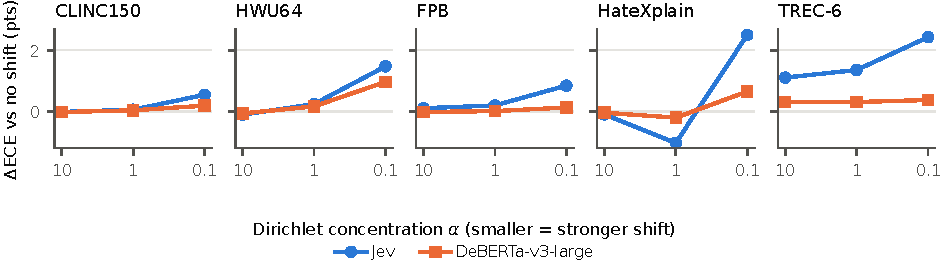
\includegraphics[width=\linewidth]{figures/fig3_shift.pdf}
  \caption{\textbf{Under stronger shift, Jev's calibration error grows more than DeBERTa-v3-large's on all five
  datasets, but this is not a zero-shot versus trained contrast: the TF-IDF classifier degrades more than Jev on two of
  them, and Tev1-4B more than Jev on FPB and TREC-6 (descriptive).}
  Change in ECE relative to a resampled no-shift control, mean over 200 Dirichlet draws per $\alpha$, raw probabilities.
  Only $\alpha=1$ is tested (\hyperref[tab:pa]{Table~\ref*{tab:pa}}); all systems in \hyperref[tab:exp2delta]{Table~\ref*{tab:exp2delta}}.}
  \label{fig:shift}
\end{figure}

\subsection{RQ3: Implicit-prior correction}
\label{sec:rq3}

\paragraph{EM with Jev's implicit prior lowers its calibration error under shift on the two datasets where that error is
highest.}
EM prior correction with Jev's implicit prior lowers Jev's ECE under shift on FPB by 2.7~points ($[-3.7,-1.6]$;
$p<0.007$; PA3) and on HateXplain by 1.8~points ($[-2.7,-0.8]$; $p<0.007$), the two datasets where Jev's unshifted ECE is
highest (0.095 and 0.279). On CLINC150 and HWU64, where its ECE is at most 0.036, the intervals lie between $-0.33$ and
$+0.54$ points; on TREC-6 the estimate is $-1.1$ points ($[-2.0,-0.3]$) but not significant after correction ($p=0.136$). Unlike PA1
and PA2, these effects keep their sign across shift scenarios: across the five other prior sets, the reduction is 1.7 to 2.5~points on FPB, 1.8 to 2.5 on HateXplain and 0.9 to 1.1 on TREC-6, with every unadjusted interval excluding zero
(\hyperref[tab:pasens]{Table~\ref*{tab:pasens}}). The FPB and HateXplain effects also exceed Jev's run-to-run variation in ECE (at most 0.6 and
1.1~points on these two datasets; \hyperref[tab:jevrepeat]{Table~\ref*{tab:jevrepeat}}). Descriptively, they appear to correct the shift rather
than Jev's label bias: on the resampled no-shift control, EM changes Jev's ECE by only $+0.1$ points on FPB and $+0.4$ on
HateXplain (descriptive; \hyperref[tab:emnoshift]{Table~\ref*{tab:emnoshift}}). The
correction is modest relative to the error it addresses: on HateXplain, Jev's mean ECE under shift falls from 0.271 to
0.254, whereas bias-corrected temperature scaling followed by EM, which needs development labels, reaches 0.071.
Descriptively, the same label-free correction lowers the shifted ECE of every zero-shot system on FPB and HateXplain, by
0.9 to 4.6~points (\hyperref[tab:exp2arms]{Table~\ref*{tab:exp2arms}}).

\paragraph{Most of the calibration gain under shift comes from calibrating on the development set (descriptive).}
The arms fall into two categories that should not be compared as alternatives: EM with the implicit prior is
\emph{label-free} and is the only option when no labelled data are available, whereas temperature scaling and BCTS+EM
are \emph{labelled} recalibration fitted on the labelled development set (the oracle uses the true target prior and is
only a reference). \hyperref[fig:arms]{Figure~\ref*{fig:arms}} and \hyperref[tab:exp2arms]{Table~\ref*{tab:exp2arms}} compare all five arms. On FPB and HateXplain, where most systems are
miscalibrated, bias-corrected temperature scaling followed by EM gives the lowest ECE under shift for 13 of the 14
system--dataset pairs, for example 0.035 for Nimble-9B on FPB against 0.271 without recalibration; the exception is
DeBERTa-v3-large on FPB, where temperature scaling alone is 0.2~points lower. Its gain is mostly the correction of
miscalibration that exists without shift: relative to its own no-shift control, the ECE of BCTS+EM still rises under shift,
by 1.5 to 3.1~points for the zero-shot systems on HateXplain, more than the raw probabilities do there, but it stays far
below the unrecalibrated level. Temperature scaling alone transfers less well: its ECE increases under shift more than
that of the raw probabilities for 31 of the 35 system--dataset pairs.

\begin{figure}[t]
  \centering
  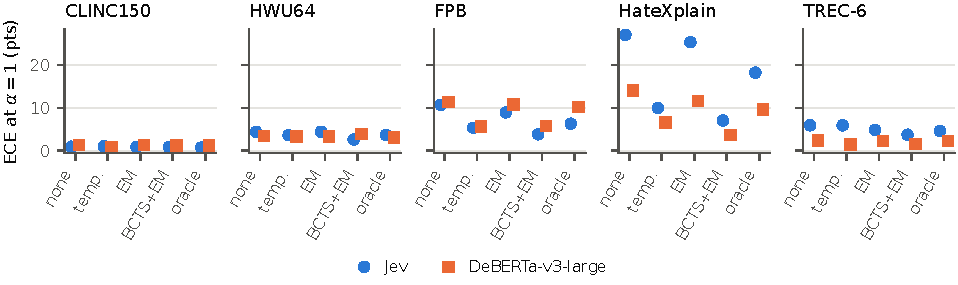
\includegraphics[width=\linewidth]{figures/fig4_arms.pdf}
  \caption{\textbf{Most of the calibration gain under shift comes from calibrating on the development set, not from
  correcting the prior (descriptive).} ECE under shift ($\alpha=1$, mean over 200 draws) for each recalibration arm.
  Label-free: EM, prior correction with the source prior (implicit for Jev, training prior for DeBERTa-v3-large).
  Labelled (fitted on the labelled development set): temp., temperature scaling; BCTS+EM, bias-corrected temperature
  scaling, then EM. Reference: oracle, true target prior (not deployable). All systems in \hyperref[tab:exp2arms]{Table~\ref*{tab:exp2arms}}.}
  \label{fig:arms}
\end{figure}
